\section{Implementation}
Um die Feldlinien darzustellen müssen diese heruntergeladen und dekomprimiert werden. Die zwei Operationen sind die Hauptverantwortlichen für die Wartezeit. Um die Wartezeit zu verkürzen, werden Feldlinien bereits im Voraus asynchron heruntergeladen. Somit sind die Daten bereits im Arbeitsspeicher, bevor die Visualisierung sie benötigt.\\
Die Wartezeit kann mit zusätzlichen Massnahmen weiter verkürzt werden Folgende Massnahmen wurden implementiert:
\begin{enumerate}
	\item Asynchrone Dekompression.
	\item Vorladen der Dekomprimierten Feldlinien.
	\item Mehrstufiges Caching.
\end{enumerate}
Die dekomprimierten Feldlinien sollen bereit stehen, bevor sie gebraucht werden.\\
Damit die Visualisierung durch das Read-Ahead dekomprimieren nicht unterbrochen wird, wird die Dekompression neu Asynchron ausgeführt. Zusätzlich führt die Asynchrone Implementation zu Performanceverbesserung, da die Dekompression paralellisiert werden kann.\\
Durch das CachingDie unkomprimierten sowie die komprimierten Feldlinien werden im Arbeitsspeicher zwischengespeichert. Wenn der Benutzer nun ''Zurückspuhlt´´ in der Visualisierung, kann im besten Fall auf unkomprimierte FEldlinien zurückgegriffen werden. Im zweitbesten muss nur noch die Dekompression erfolgen. Im schlechtesten müssen wieder Feldlinien hinzugeladen werden.Sonderfall, bei sehr langsamen verbindungen möchte man alle Daten cachen: Möglichkeit alle komprimierten Feldlinien im Speicher zu cachen.\\

was nicht gemacht wurde, mehrere Dateien zusammengefasst.

\subsection{Software Architektur}
\begin{figure}[!htbp]
	\center
	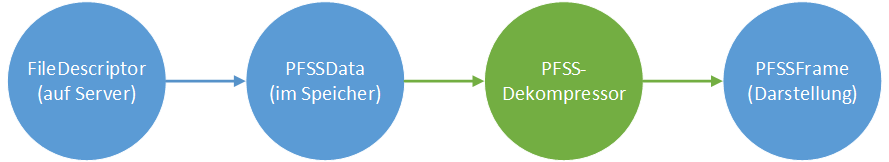
\includegraphics[width=0.8\textwidth,height=6cm,keepaspectratio]{./pictures/implementation/dataflow.png}
	\caption{Zustandsdiagramm der Feldliniendatn}
	\label{implementation:architektur:datenfluss}
\end{figure}
Die Daten der Feldlinien durchlaufen im JHelioviewer vier Zustände, welche durch vier Klassen abgebildet wurde. Die Klassen sowie die Zustandswechsel sind in Abbildung \ref{implementation:architektur:datenfluss} dargestellt. Die Klasse ''FileDescriptor´´ repräsentiert eine Aufnahme von Feldlinien auf dem Server. In diesem Zustand sind die Daten bereit für das Herunterladen. Die folgende Klasse ''PFSSData´´ symbolisiert Feldlinien, welche in den lokalen Arbeitsspeicher geladen wurden. In diesem Zustand sind die Daten noch komprimiert und nicht bereit für eine Visualisierung. Für das Herunterladen ist ebenfalls die ''PFSSData´´ Klasse zuständig. ''PFSSDekompressor´´ ist ein Zwischenzustand und stellt den Wechsel von komprimierten zu unkomprimierten Daten dar. Da der Zustandswechsel aufwändig ist, wird es durch eine eigene Klasse abgebildet. Die letzte Klasse ''PFSSFrame´´ repräsentiert die dekomprimierten Feldlinien. In diesem Zustand sind die Daten bereit für die Darstellung. Die Darstellung wird ebenfalls von der ''PFSSFrame´´ Klasse übernommen.

\subsubsection{Mehrstufiges Read Ahead und Caching}
Um den Flaschenhals herunterladen und Dekomprimieren zu umgehen, wird ein mehrstufiges Read-Ahead und Caching eingeführt. Es soll ein Read Ahead und Caching für die unkomprimierten ''PFSSFrame´´ Feldllinien und eines für die ''PFSSData´´ Objekte implementiert werden. Für das wurde folgende Klassen implementiert:
(Klassendiagramm)
Die Klasse ''Framemanager´´ stellt die erste Stufe dar des Read-Aheads dar. Sie ist dafür zuständig, das aktuelle ''PFSSFrame´´ Objekt im speicher zu behalten und falls welche Fehlen, sie vom FrameCache anzufordern. ''PFSSFrame´´ Objekte müssen jeweils Speicher auf der Grafikkarte alloziieren und selbst abräumen. Der Manager gibt den Objekten die Chance sich vor dem Darstellen zu inizialisieren und stellt sicher, dass die Ressourcen der Grafikkarte abgeräumt wurden. Dür das Caching der Frame-Objekte ist die Klasse FrameCache zuständig.\\
Das Preloading und Caching der PFSSData Objekte wird von der Klasse DataCache übernommen. Das Preloading ist als zweite Cache-Instanz umgesetzt. Hier braucht es keine Kontrolle darüber, wann ein Objekt aus einem Cache entladen wird. Der Garbage-Collector verwaltet alle Ressourcen des Data-Objekts.\\
[\baselineskip] 
Der Cache arbeitet mit einer FiFo queue für die entscheidung, wann ein Objekt aus dem cache entladen wird. Der JHelioviewer fragt im allgemeinen Fall sequenzell nach den Datenobjekten. Das älteste Objekt ist meistens das, welches am längsten nicht mehr gebraucht wird.\\
Der LRU-Cache funktioniert gut, wenn die anzahl Objekte deutlich grösser ist, als der Cache zu halten mag. Der LRU-Cache versagt aber beim Wrap-Around. Wenn es aber $n$ Objekte gibt und der Cache $n-1$ Objekte speichern kann, so löscht er immer das Nächste Objekt, welches gebraucht wird. 

\subsubsection{Asynchrone Aufrufe mittels Executor Services}
Um vom Preload und Caching sinnvoll gebrauch zu machen, muss die Dekompression und das Herunterladen der Feldlinien asynchron implementiert sein. Dazu müssen alle Klassen aus Abbildung \ref{implementation:architektur:datenfluss} threadsafe sein.
Die Klasse FileDescriptor ist einfach, diese ist Immutable und somit Threadsafe.
PFSSData und Frame threadsafe, data + compressor implementieren runnable
Nun Creators verwenden den Executor Service für bla


